% ----------------------------------------------------------------
% AMS-LaTeX Paper ************************************************
% **** -----------------------------------------------------------
\documentclass{amsart}
\usepackage{graphicx}
% ----------------------------------------------------------------
\vfuzz2pt % Don't report over-full v-boxes if over-edge is small
\hfuzz2pt % Don't report over-full h-boxes if over-edge is small
% THEOREMS -------------------------------------------------------
\newtheorem{thm}{Theorem}[section]
\newtheorem{cor}[thm]{Corollary}
\newtheorem{lem}[thm]{Lemma}
\newtheorem{prop}[thm]{Proposition}
\theoremstyle{definition}
\newtheorem{defn}[thm]{Definition}
\theoremstyle{remark}
\newtheorem{rem}[thm]{Remark}
\numberwithin{equation}{section}
% MATH -----------------------------------------------------------
\newcommand{\norm}[1]{\left\Vert#1\right\Vert}
\newcommand{\abs}[1]{\left\vert#1\right\vert}
\newcommand{\set}[1]{\left\{#1\right\}}
\newcommand{\Real}{\mathbb R}
\newcommand{\eps}{\varepsilon}
\newcommand{\To}{\longrightarrow}
\newcommand{\BX}{\mathbf{B}(X)}
\newcommand{\A}{\mathcal{A}}
% ----------------------------------------------------------------
\begin{document}

\title{Complex Networks  - Spring 2024\\{\bf Homework 4}}%
\author{Instructor: Jia Liu \\ Solution by: Renan Monteiro Barbosa}%
\date{04/20/2025}

%\dedicatory{}%
%\commby{}%
% ----------------------------------------------------------------

\maketitle
% ----------------------------------------------------------------
\begin{itemize}
\item DUE on  04/20/2025 11:59pm C.T.
\item This is a group porject. Each group only needs to submit one file.
\item All files should be typed. 
\item Please name your file as follows: $LastnameInitials-MAP6306quiz1.pdf$.If your name is  David Roberts, file name is $RobertsAD-MAP6306quiz1.pdf$.
\item Try to keep the file size less than 4MB.
\item You can resubmit the quiz if you want. Please specify which one is the one to be graded. Otherwise I will grade the most recent version.
\item DO NOT EMAIL me the quiz. All quizzes are submitted via Canvas.
\end{itemize}


\clearpage
\begin{enumerate}

%---------------------------------------------------------------------------------
% ##############################################################################
% Problem 1
% ##############################################################################

\item Consider following data sets (you can download the data here https://websites.umich.edu/~mejn/netdata/).
\begin{enumerate}
\item Zachary's karate club
\item American College football
\item Power grid
\end{enumerate}

\vspace{2cm}

Report the questions below for each network:
\begin{enumerate}
\item Use Gephi to plot the network. Make sure to use centrality and communities so that you can show the properties of the network.
\item Use Gephi to find how many communities this network has. 
\item What is the modularity for the community detection?
\end{enumerate}
\end{enumerate}

\vspace{0.5 cm}

% #############################################
% Answers
% #############################################

\textbf{Answers:}

\vspace{0.5 cm}

\begin{enumerate}
    \item Use Gephi to plot the network. \vspace{0.5 cm}
    \begin{enumerate}
        % #############################################
        % Problem 1-a --- Zachary’s karate club
        % #############################################
        \item Plot \textbf{Zachary's karate club} network with Gephi. \vspace{0.5 cm}
        \centering
        \begin{minipage}{1\textwidth}
        \centering
        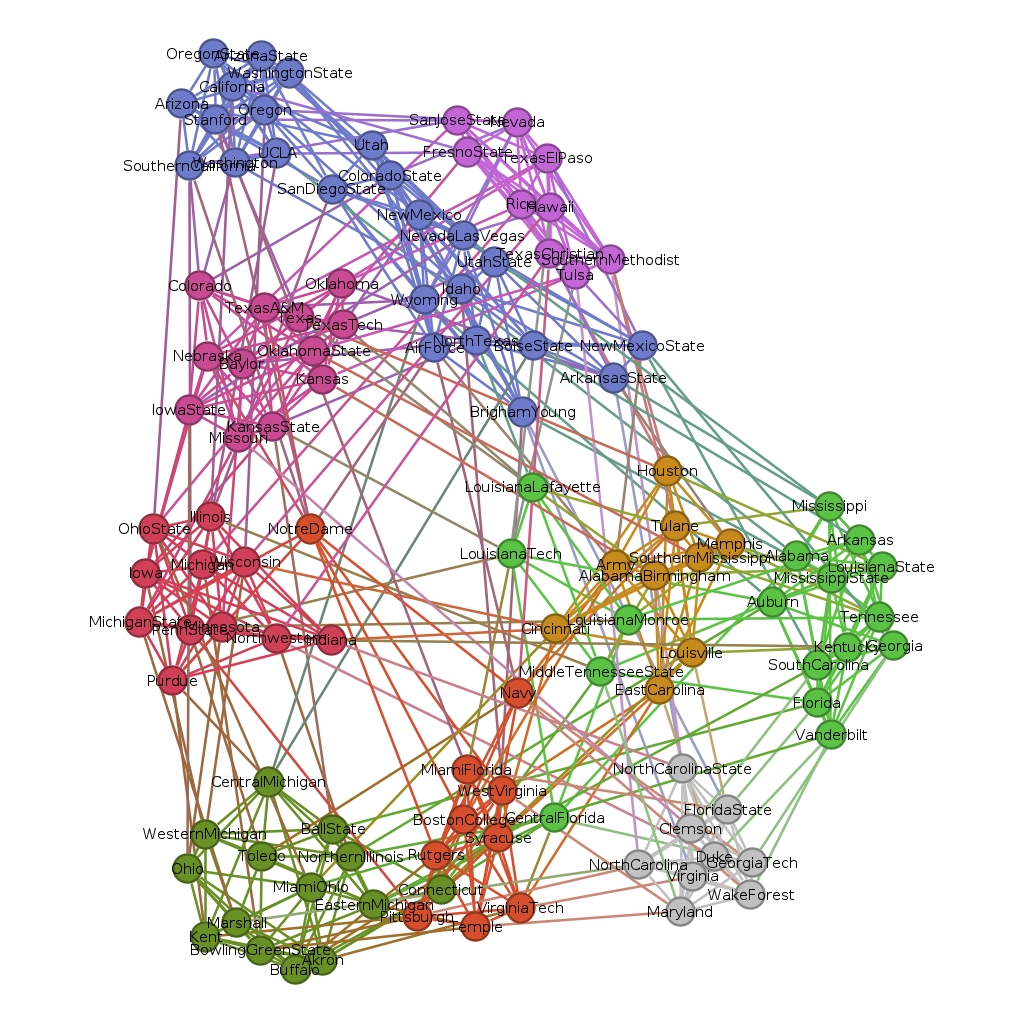
\includegraphics[width=0.8\textwidth]{images/football_v0.png} % Replace with your image file
        \end{minipage}

        Each node represents a member of the karate club. This includes the instructor, the administrator, and other club members. 
        
        Each edge represents a mutual social interaction between two members. 

        \vspace{0.5 cm}

        % #############################################
        % Problem 1-a --- American College football
        % #############################################
        \item Plot \textbf{American College football} network with Gephi. \vspace{0.5 cm}
        \centering
        \begin{minipage}{1\textwidth}
        \centering
        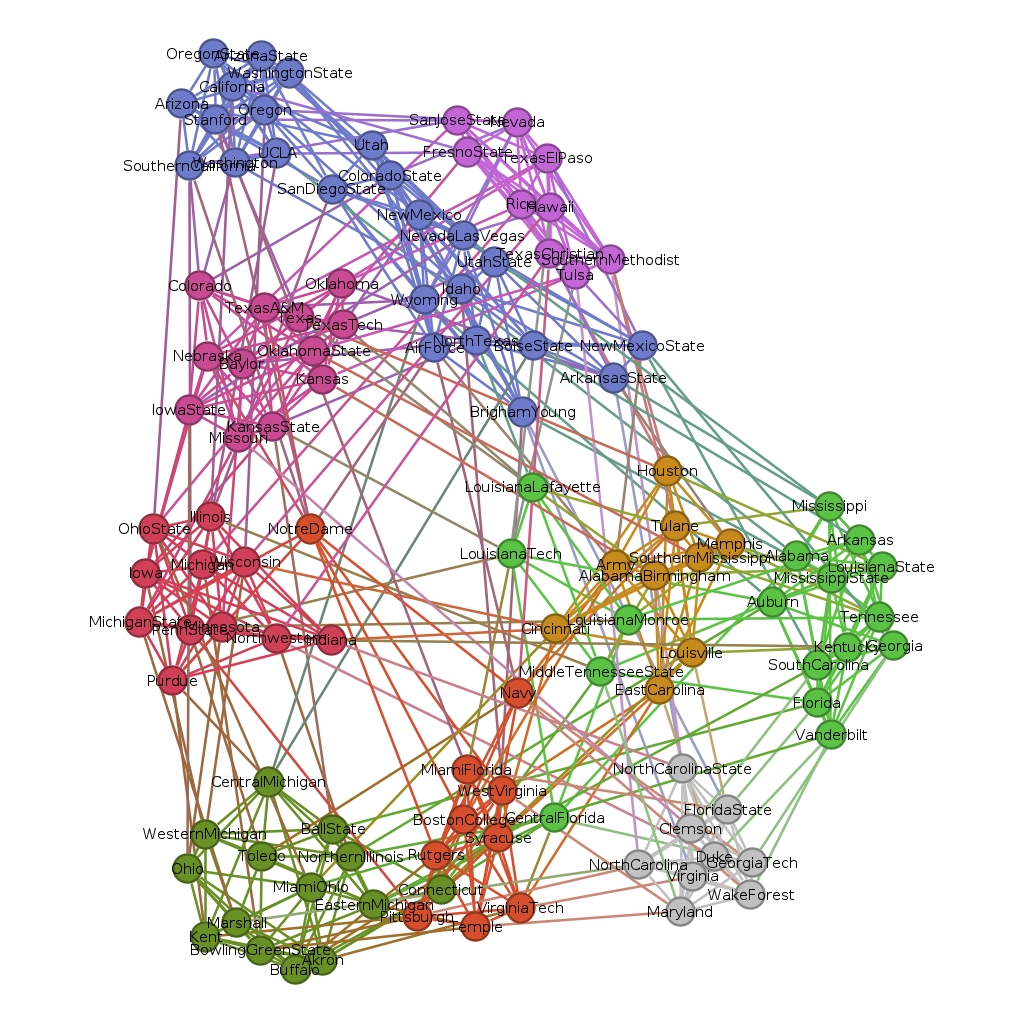
\includegraphics[width=0.8\textwidth]{images/football_v0.png} % Replace with your image file
        \end{minipage}

        % \begin{figure}[h]
        % 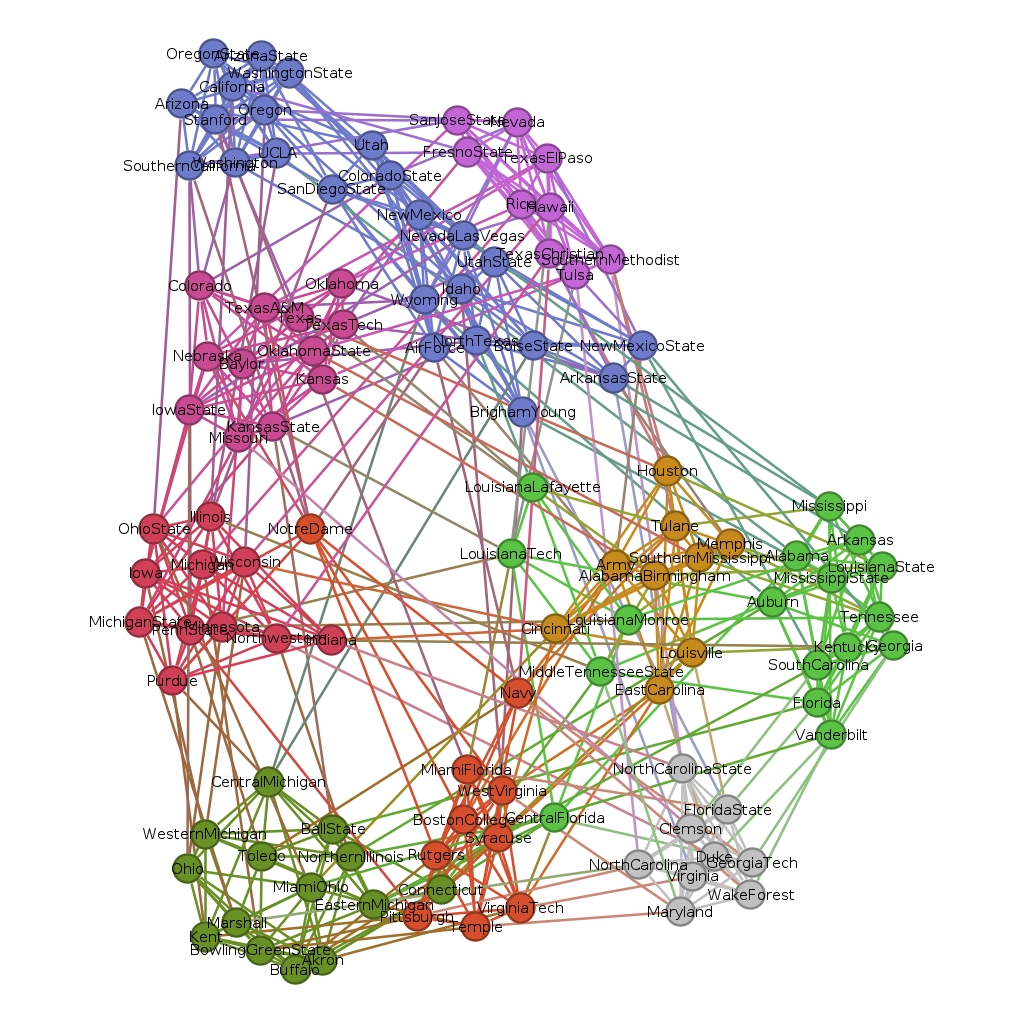
\includegraphics[width=0.8\linewidth]{images/football_v0.png}
        % \end{figure}

        The football network represents games played between Division IA college teams during regular season in Fall 2000. The nodes have calues that indicate to which conferences they belong.
        
        We can observe that the algorithm detected 9 communities, which is close to the actual 12 NCAA conferences. This indicates that there are also inter-conference games. 

        \vspace{0.5 cm}

        % #############################################
        % Problem 1-a --- Power grid
        % #############################################
        \item Plot \textbf{Power grid} network with Gephi. \vspace{0.5 cm}

        The \textbf{Power grid} network represents the topology of the western states power grid of the United States. We can observe that tehre are tighly clustered groups which demonstrates that the way how the network is organized is dependent on the infrastructure and their geographical location and importance most likely.

        There are 4941 nodes and 6594 edges

        \vspace{0.5 cm}

    \end{enumerate}
    % #############################################
    % #############################################
    % #############################################
    % #############################################
    \item Use Gephi to find how many communities this network has. \vspace{0.5 cm}
    \begin{enumerate}
        % #############################################
        % Problem 1-b --- Zachary’s karate club
        % #############################################
        \item Use Gephi to find how many communities there are in the \textbf{Zachary's karate club} network. \vspace{0.5 cm} 

        There are 4 communities in the \textbf{Zachary's karate club} \vspace{0.5 cm}

        % #############################################
        % Problem 1-b --- American College football
        % #############################################
        \item Use Gephi to find how many communities there are in the \textbf{American College football} network. \vspace{0.5 cm}

        There are 9 communities in the \textbf{American College football} \vspace{0.5 cm}

        % #############################################
        % Problem 1-b --- Power grid
        % #############################################
        \item Use Gephi to find how many communities there are in the \textbf{Power grid} network. \vspace{0.5 cm}

        There are 39 communities in the \textbf{Power grid} \vspace{0.5 cm}

    \end{enumerate}
    % #############################################
    % #############################################
    % #############################################
    % #############################################
    \item What is the modularity for the community detection? \vspace{0.5 cm}
    \begin{enumerate}
        % #############################################
        % Problem 1-c --- Zachary’s karate club
        % #############################################
        \item What is the modularity for the community detection in the \textbf{Zachary’s karate club} network? \vspace{0.5 cm}

        Modularity Score: 0.390 

        \vspace{0.5 cm}

        % #############################################
        % Problem 1-c --- American College football
        % #############################################
        \item What is the modularity for the community detection in the \textbf{American College football} network? \vspace{0.5 cm}

        Modularity Score: 0.604

        \vspace{0.5 cm}

        % #############################################
        % Problem 1-c --- Power grid
        % #############################################
        \item What is the modularity for the community detection in the \textbf{Power grid} network? \vspace{0.5 cm}

        Modularity Score: 0.926 

        \vspace{0.5 cm}

    \end{enumerate}
    % #############################################
    % #############################################
    % #############################################
    % #############################################
\end{enumerate}

\end{document}
% ----------------------------------------------------------------
